\section{Motivation}
\label{sec:motivation}
Every time we train ML models on the same dataset, we can achieve different accuracies. Taking figure \ref{fig:motiv} as an example, a user obtains various accuracy values while training the same model on one dataset. \footnote{\small \url{https://stackoverflow.com/questions/55775450/}}.
\begin{figure}[h]
	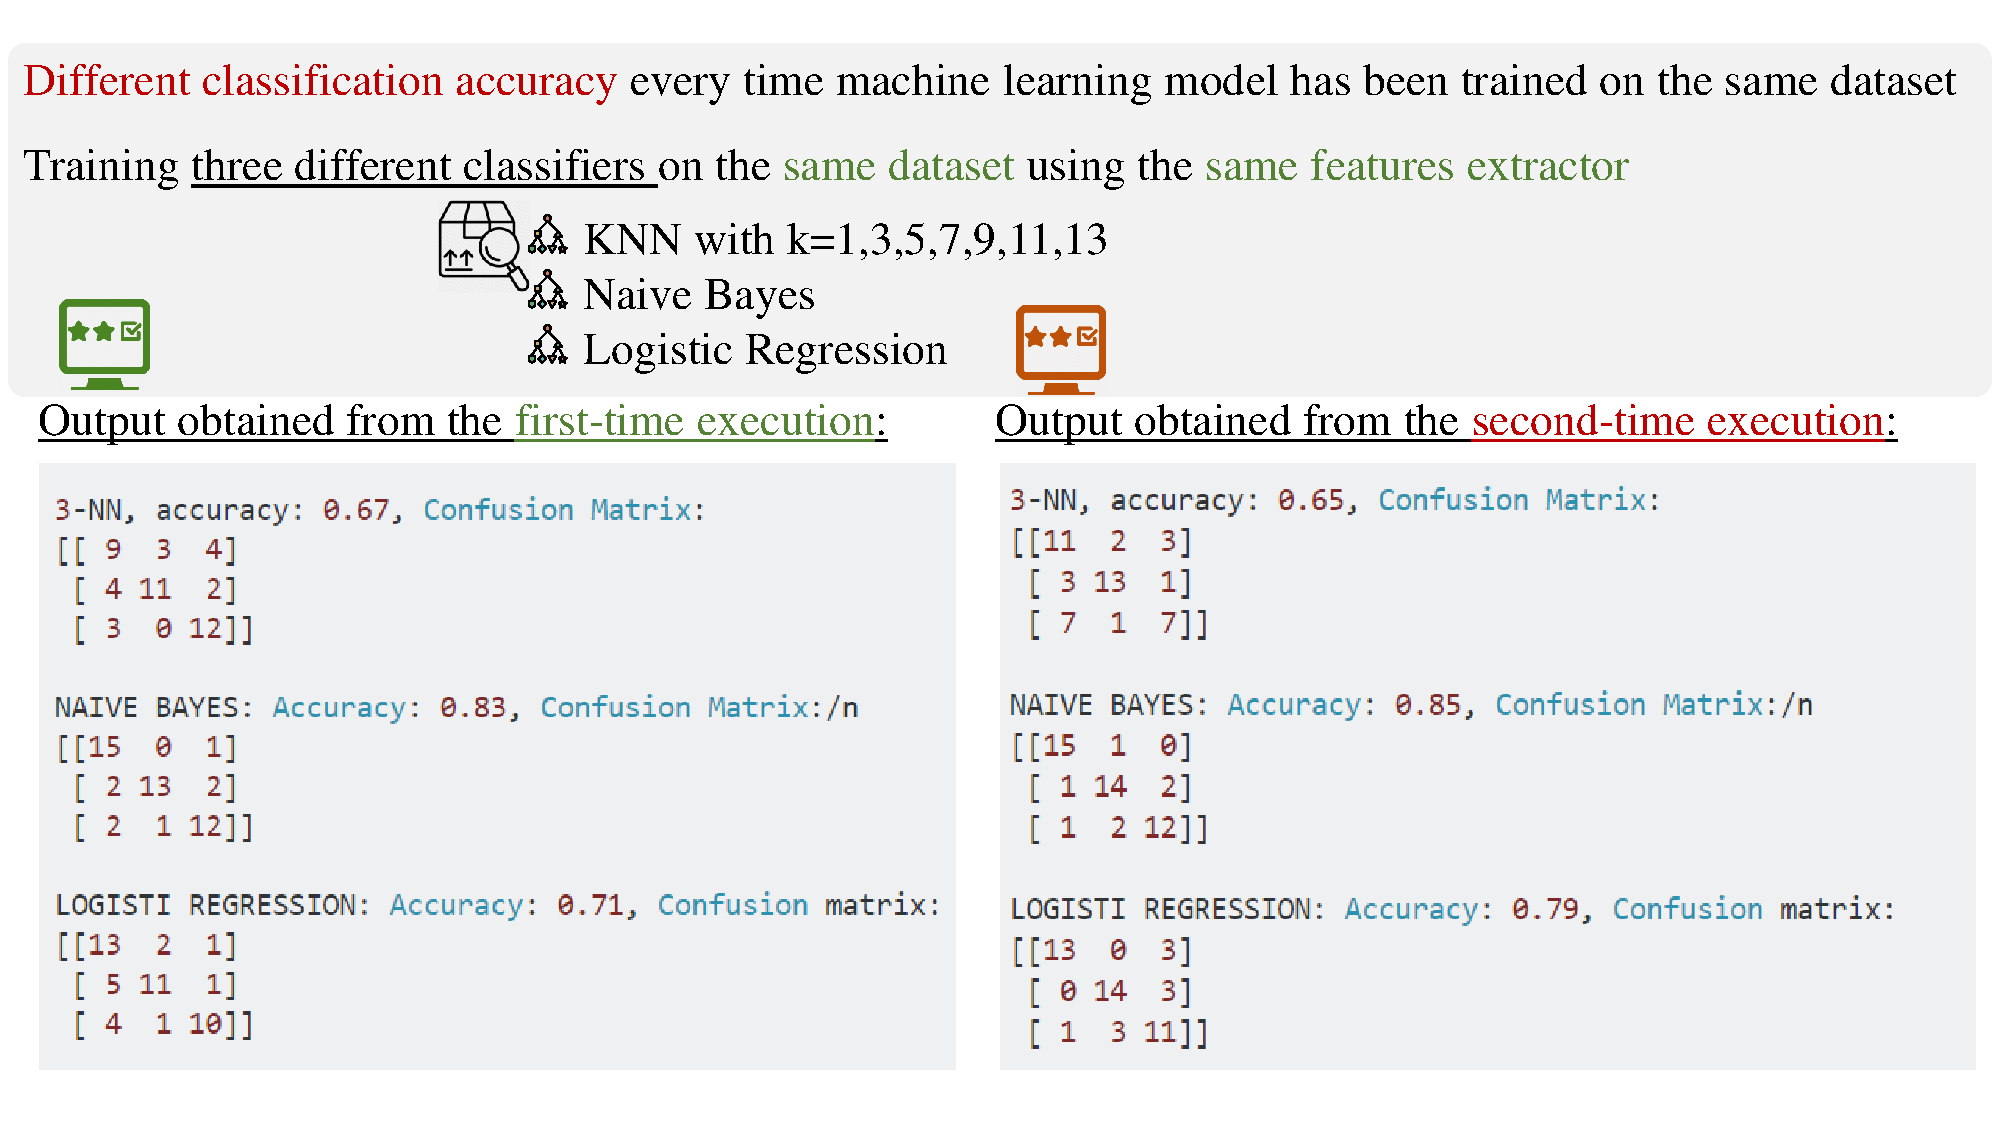
\includegraphics[width=\linewidth]{motivfigure.pdf}
	\caption{Example of different accuracy on each execution using same experimental setup}
	\label{fig:motiv}
	%\vspace{15pt}
\end{figure}

In this scenario, different classification accuracy has been obtained with every execution of a machine learning model that has been trained on the same dataset. Three different classifiers e.g., k-nearest neighbors, Naive Bayes, and Logistic Regression have been compared using the accuracy of each model. With every execution, these models have been trained with the same experimental setup, different values of accuracy for each model have been obtained as illustrated in Figure \ref{fig:motiv}. These results in a lack of trustworthiness of an ML-based model. Currently, we still do not have an appropriate answer to the results produced by ML models. However, we do know that initial bias and weight have a contribution to the final results of an ML model. Moreover, one of the factors which cause the different accuracies of ML models on the same dataset is different initial bias and weight. The obvious question would be can we increase the accountability of an ML model by obtaining the best accuracy among the possible accuracies produced by this model? He\etal \cite{he2015delving} also mentions that an ML model can be obstructed by bad initializations of weight and bias. 
\begin{figure*}{}
	\centering
	
	\begin{subfigure}[b]{.30\linewidth}{}
		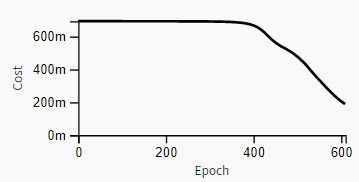
\includegraphics[keepaspectratio = True, scale = 0.40]{figures/small.png}
		\centering
		\caption{Too small initialization}
		\vspace{2.0em}
		\label{fig:sml}
	\end{subfigure}
	\begin{subfigure}[b]{.30\linewidth}
		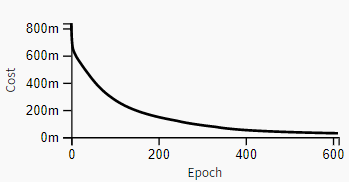
\includegraphics[keepaspectratio = True, scale = 0.40]{figures/apr.png}
		\caption{Appropriate initialization}
		\vspace{2.0em}
		\label{fig:apr}
	\end{subfigure}
	\begin{subfigure}[b]{.30\linewidth}
		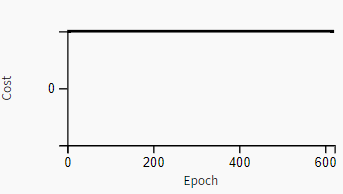
\includegraphics[keepaspectratio = True, scale = 0.40]{figures/lrg.png}
		\caption{Too large initialization}
		\vspace{2.0em}
		\label{fig:lrg}
	\end{subfigure}
	
	
	\caption{Performance of a ML model on a dataset with different initializations}
	\label{fig:results}
\end{figure*}

Figure \ref{fig:results} show the performance of a ML model on a dataset with different initializations using the setup \footnote{\small \url{https://www.deeplearning.ai/ai-notes/initialization/}}. Particularly, if we select too small initialization, the model will take a long time to converge, whereas if we choose too large initialization, the model will never converge. Therefore, selecting an appropriate initialization is crucial for the performance of a deep neural model. In this project, we propose a method to make the DNN model more accountable by select appropriate initializations of weight and bias. 
%\small
%\begin{lstlisting}[language=Python, caption=Motivating example of model verification to interpret accuracy for accountable ML]
%//The first time execution of a CNN code gives this output:
%3-NN, accuracy: 0.67, Confusion Matrix:
%[[ 9  3  4]
%[ 4 11  2]
%[ 3  0 12]]
%
%NAIVE BAYES: Accuracy: 0.83, Confusion Matrix:/n
%[[15  0  1]
%[ 2 13  2]
%[ 2  1 12]]
%
%LOGISTIC REGRESSION: Accuracy: 0.71, Confusion matrix:
%[[13  2  1]
%[ 5 11  1]
%[ 4  1 10]]
%
%\\ The second time execution of the same code returns:
%3-NN, accuracy: 0.65, Confusion Matrix:
%[[11  2  3]
%[ 3 13  1]
%[ 7  1  7]]
%
%NAIVE BAYES: Accuracy: 0.85, Confusion Matrix:/n
%[[15  1  0]
%[ 1 14  2]
%[ 1  2 12]]
%
%LOGISTIC REGRESSION: Accuracy: 0.79, Confusion matrix:
%[[13  0  3]
%[ 0 14  3]
%[ 1  3 11]]
%\end{lstlisting}
